\documentclass[a4paper,12pt,oneside]{book}
\usepackage{polski}
\usepackage[utf8]{inputenc}
\usepackage{graphicx}
\graphicspath{{./images}}
\usepackage[shortlabels]{enumitem}
\usepackage{amssymb}
\usepackage{amsmath}
\usepackage{indentfirst}

\usepackage{tikz}
%\usepackage{etoolbox} % for \ifthen
\usepackage{listofitems} % for \readlist to create arrays
\usetikzlibrary{arrows.meta} % for arrow size
\usepackage[outline]{contour} % glow around text
\contourlength{1.4pt}

\tikzset{>=latex} % for LaTeX arrow head
\usepackage{xcolor}
\colorlet{myred}{red!80!black}
\colorlet{myblue}{blue!80!black}
\colorlet{mygreen}{green!60!black}
\colorlet{myorange}{orange!70!red!60!black}
\colorlet{mydarkred}{red!30!black}
\colorlet{mydarkblue}{blue!40!black}
\colorlet{mydarkgreen}{green!30!black}
\tikzstyle{node}=[thick,circle,draw=myblue,minimum size=22,inner sep=0.5,outer sep=0.6]
\tikzstyle{node in}=[node,green!20!black,draw=mygreen!30!black,fill=mygreen!25]
\tikzstyle{node hidden}=[node,blue!20!black,draw=myblue!30!black,fill=myblue!20]
\tikzstyle{node convol}=[node,orange!20!black,draw=myorange!30!black,fill=myorange!20]
\tikzstyle{node out}=[node,red!20!black,draw=myred!30!black,fill=myred!20]
\tikzstyle{connect}=[thick,mydarkblue] %,line cap=round
\tikzstyle{connect arrow}=[-{Latex[length=4,width=3.5]},thick,mydarkblue,shorten <=0.5,shorten >=1]
\tikzset{ % node styles, numbered for easy mapping with \nstyle
	node 1/.style={node in},
	node 2/.style={node hidden},
	node 3/.style={node out},
}
\def\nstyle{int(\lay<\Nnodlen?min(2,\lay):3)} % map layer number onto 1, 2, or 3

\def\shrug{\texttt{\raisebox{0.75em}{\char`\_}\char`\\\char`\_\kern-0.5ex(\kern-0.25ex\raisebox{0.25ex}{\rotatebox{45}{\raisebox{-.75ex}"\kern-1.5ex\rotatebox{-90})}}\kern-0.5ex)\kern-0.5ex\char`\_/\raisebox{0.75em}{\char`\_}}}

\renewcommand\thesubsection{\arabic{subsection}}

\begin{document}
	\chapter*{Odpowiedzi na pytania z egzaminu licencjackiego}
	\subsection{Wektory i macierze – definicje i podstawowe operacje.}
	
	Macierz to układ liczb, symboli lub wyrażeń zapisanych w postaci prostokątnej tablicy. W algebrze liniowej macierze wprowadza się często jako sposób skondensowanego zapisu układów równań liniowych, co ma na celu wyeliminowanie powtarzających się elementów standardowej notacji układów równań tego rodzaju z wieloma niewiadomymi. Macierze pozwalają również na reprezentowanie przekształceń liniowych w sposób umożliwiający przeprowadzanie obliczeń. Ponieważ wiele przekształceń geometrycznych (jak na przykład obroty przestrzeni $\mathbb {R} ^{n}$ wokół początku układu współrzędnych) są przekształceniami liniowymi, macierze znajdują zastosowanie w geometrii analitycznej i grafice komputerowej.
	
	Przykład zapisu macierzy $3\times 3$
	$ \begin{bmatrix}
		8 & 3 & 2 \\
		5 & 4 & 1 \\
		2 & 9 & 0 
	\end{bmatrix}  $
	
	Macierze ${\displaystyle \mathbf {A} =[a_{ij}]}$ i ${\displaystyle \mathbf {B} =[b_{ij}]}$ uważa się za równe, jeśli mają ten sam typ i równe odpowiadające sobie elementy, tzn. dla każdej możliwej pary $i,j$ zachodzi ${\displaystyle a_{ij}=b_{ij}.}$\\
	
	Sumę macierzy $\mathbf{A}$ i $\mathbf{B}$ definiuje się „po współczynnikach”, tzn. za pomocą wzoru $\mathbf {A+B} =[a_{ij}+b_{ij}]$ dla wszystkich $i,j.$ Z definicji wynika (ale można napisać wprost), że można dodawać macierzy tylko o takich samych wymiarach.
	
	\begin{center}
		$ \begin{bmatrix}
			8 & 3 & 2 \\
			5 & 4 & 1 \\
			2 & 9 & 0 
		\end{bmatrix} + 
	\begin{bmatrix}
		2 & 2 & 6 \\
		3 & 5 & 7 \\
		1 & 0 & 4 
	\end{bmatrix} = 
\begin{bmatrix}
	10 & 5 & 8 \\
	8 & 10 & 8 \\
	3 & 9 & 4 
\end{bmatrix}$
	\end{center}
	
	Mnożenie przez skalar macierzy $\mathbf{A}$ oraz liczby $c$ również definiuje się „po współczynnikach”, czyli $c\mathbf {A} =[ca_{ij}]$ dla dowolnych $ i,j.$\\
	\begin{center}
		$ 2 * \begin{bmatrix}
			8 & 3 & 2 \\
			5 & 4 & 1 \\
			2 & 9 & 0 
		\end{bmatrix} = 
	\begin{bmatrix}
		16 & 6 & 4 \\
		10 & 8 & 2 \\
		4 & 18 & 0 
	\end{bmatrix}$
	\end{center}

	Działanie mnożenia macierzy jest zdefiniowane najczęściej jako tzw. iloczyn Cauchy'ego: dla dla macierzy ${\mathbf  A}$ typu $m\times n$ oraz $\mathbf{B}$ typu $n \times p$ dany jest on jako taka macierz $\mathbf C$ typu $m\times p,$ oznaczana $\mathbf {AB} ,$ dla której
	
	$c_{ij}=a_{i1}b_{1j}+a_{i2}b_{2j}+\dots +a_{in}b_{nj}$ dla dowolnych $i,j.$\\
	
	Mnożenie to jest łączne ($A(BC)=(AB)C$), ale nie jest przemienne ($AB \neq BA$).\\
	
		\begin{center}
		$\begin{bmatrix}
			2 & 3 & 7 \\
			6 & 1 & 2 
		\end{bmatrix} 
		\begin{bmatrix}
			1 \\
			0\\
			5 
		\end{bmatrix} = 
		\begin{bmatrix}
		2 * 1 + 3 * 0 + 7 * 5\\
		6 * 1 + 1 * 0 + 2 * 5
	\end{bmatrix}=
	\begin{bmatrix}
		37\\
		16
	\end{bmatrix}$
	\end{center}
	
	
	
	\begin{figure}[h!]
		\centering
		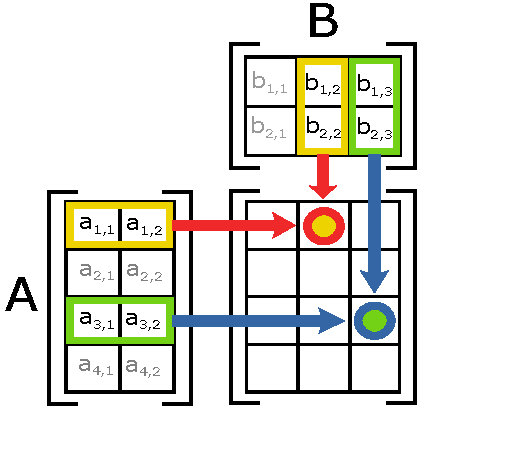
\includegraphics[scale=0.8]{Matrix_multiplication_diagram_2.pdf}
		\caption{Schemat mnożenia macierzy A i B}
	\end{figure}

	Elementem neutralnym mnożenia macierzy przez siebie jest macierz diagonalna, zawierająca na swojej przekątnej same jedynki.
			\begin{center}
		$\begin{bmatrix}
			2 & 3 & 7 \\
			6 & 1 & 2 
		\end{bmatrix} 
		\begin{bmatrix}
			1 & 0 & 0 \\
			0 & 1 & 0\\
			0 & 0 & 1 
		\end{bmatrix} = 
		\begin{bmatrix}
			2 & 3 & 7 \\
			6 & 1 & 2 
		\end{bmatrix}$ 
	\end{center}

	Przestawienie bądź transpozycja danej macierzy $\mathbf {A}$, tzn. zamiana jej kolumn i wierszy miejscami (z zachowaniem kolejności). Macierz transponowaną lub przestawioną względem macierzy $\mathbf  A$ definiuje się jako macierz
	
	$\mathbf {A} ^{\mathrm {T} }=[a_{ji}]$ dla wszystkich $i,j,$ przy czym $(\mathbf {AB} )^{\mathrm {T} }=\mathbf {B} ^{\mathrm {T} }\mathbf {A} ^{\mathrm {T} }$ oraz $\left(\mathbf {A} ^{\mathrm {T} }\right)^{\mathrm {T} }=\mathbf {A} .$\\
	
	Wyznacznikiem $\det(\mathbf {A} )$ lub $|\mathbf {A} |$ macierzy kwadratowej $\mathbf  A$ nazywa się liczbę kodującą pewne właściwości przekształcenia $\mathrm {A}$ reprezentowanego przez tę macierz. \\
	
	Wyznacznik macierzy stopnia drugiego dany jest wzorem
	\begin{center}
			${\displaystyle \det {\begin{bmatrix}a&b\\c&d\end{bmatrix}}=ad-bc.}$\\
	\end{center}

	
	
	Wektor jest macierzą o wymiarach $n\times 1$. Reprezentuje on punkt w przestrzeni $\mathbb{R}^n$. Jego podstawowe trzy cechy to:
	\begin{itemize}
		\item długość - czasami inaczej zwana modułem lub wartością
		\item kierunek - kierunek prostej zawierającej wektor
		\item zwrot - grot strzałki
	\end{itemize}

	\begin{figure}[h!]
		\centering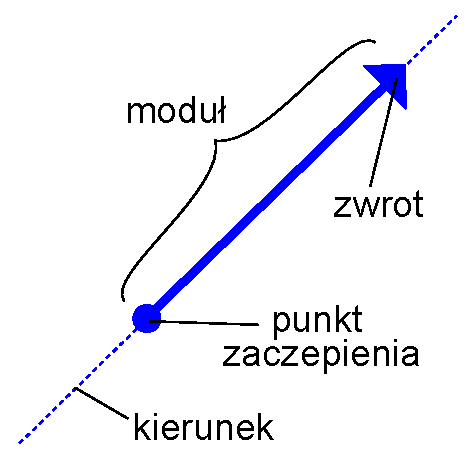
\includegraphics[scale=0.7]{Wektor_by_Zureks.pdf}
		\caption{Ilustracja wektora}
	\end{figure}

	Dodawanie oraz mnożenie przez skalar wektora jest zdefiniowane w ten sam sposób jak w przypadku macierzy. \\\\\\
	
	
	Iloczyn skalarny dwóch wektorów to \textbf{liczba}, którą obliczamy dodając iloczyny odpowiednich współrzędnych.
	
	\begin{center}
		$\vec{a}=[2,1,3], \vec{b}=[4,1,2]$\\
		$\vec{a}\circ\vec{b} = 2*4 + 1*1 + 3*2 = 15$
	\end{center}

	Iloczyn skalarny możemy również obliczyć znając długości wektorów $|\vec{a}|$ i $|\vec{b}|$ oraz kąt $\alpha$ między nimi:
	
	\begin{center}
		$\vec{a}\circ\vec{b}=\|\vec{a}\|*\|\vec{b}\|*\cos\alpha$
	\end{center}

	Długość wektora $\vec{a}$ może być zdefiniowana jako pierwiastek iloczynu skalarnego z samym sobą. 
	
	\begin{center}
		$\|\vec{a}\|=\sqrt{\vec{a}\circ\vec{a}}$
	\end{center}

Iloczyn wektorowy - działanie dwuargumentowe przyporządkowujące parze wektorów przestrzeni $\mathbb{R}^3$ pewien wektor tej przestrzeni.\\

Iloczyn wektorowy $\mathbf {a} \times \mathbf {b}$ wektorów $\mathbf a $ i $ \mathbf  b$ określa się następująco:
\begin{itemize}
	\item jeśli wektory $\mathbf{a}$ i $\mathbf{b}$ są liniowo zależne, to $\mathbf{a}\times\mathbf{b}=0$
	\item jeśli wektory $\mathbf{a}$ i $\mathbf{b}$ nie są liniowo zależne, to $\mathbf{a}\times\mathbf{b}=\mathbf{c}$, gdzie $\mathbf{c}$ jest wektorem prostopadłym do płaszczyzny wyznaczonej przez $\mathbf{a}$ i $\mathbf{b}$.
\end{itemize}

\subsection{Funkcje skrótu (mieszające) i ich zastosowania.}
Funkcja skrótu, funkcja mieszająca lub funkcja haszująca – funkcja przyporządkowująca dowolnie dużej liczbie krótką wartość o stałym rozmiarze, tzw. skrót nieodwracalny.\\

W informatyce funkcje skrótu pozwalają na ustalenie krótkich i łatwych do weryfikacji sygnatur dla dowolnie dużych zbiorów danych. Sygnatury mogą chronić przed przypadkowymi lub celowo wprowadzonymi modyfikacjami danych (sumy kontrolne), a także mają zastosowania przy optymalizacji dostępu do struktur danych w programach komputerowych (tablice mieszające).\\

Szczególną podgrupą funkcji skrótu są funkcje uznawane za bezpieczne do zastosowań kryptologicznych (jak np. SHA-3). Kryptograficzna funkcja skrótu powinna spełniać kombinację następujących kryteriów, w zależności od zastosowania:\\
\begin{itemize}
	\item Odporność na kolizje (collision resistance) – brak praktycznej możliwości wygenerowania dwóch dowolnych wiadomości o takim samym skrócie
	\item Odporność na kolizje konkretnych wiadomości (target collision-resistance, preimage resistance) pierwszego i drugiego rzędu – brak praktycznej możliwości wygenerowania wiadomości o takim samym skrócie jak wskazana wiadomość
	\item Jednokierunkowość (one-wayness) – brak możliwości wnioskowania o wiadomości wejściowej na podstawie wartości skrótu. Zmiana dowolnego pojedynczego bitu wiadomości powinna zmieniać średnio połowę bitów skrótu w sposób, który nie jest istotnie podatny na kryptoanalizę różnicową.
\end{itemize}

Przykładowe funkcje skrótu to SHA-1 (SHA128), SHA-2 (SHA256), SHA-3(SHA512), MD5.

\setcounter{subsection}{5}
\subsection{Sposoby cyfrowej reprezentacji liczby całkowitej i rzeczywistej.}

\subsubsection{Liczby całkowite}

\subparagraph{Kod \text{ZM} (kod znak-moduł)}

Sprawa w kodzie ZM jest w miarę prosta i klarowna. Najstarszy bit $b_{n-1}$ dla n-bitowej liczby jest bitem znaku i określa czy liczba jest dodatnia czy ujemna:
\begin{itemize}
	\item 0 - liczba dodatnia,
	\item 1 - liczba ujemna.
\end{itemize}

Bity od $b_{n-1}$ do $b_0$ odpowiadają za kodowanie wartości samej liczby. Wzór na obliczenie wartości liczby zakodowanej w \textbf{ZM}:
\begin{center}
	$L_{ZM} = (-1)^{b_{n-1}} \cdot (b_{n-2}2^{n-2} + ... + b_22^2 + b_12^1 + b_02^0)$
\end{center}

Przykładowe kodowanie liczby na ośmiu bitach w kodzie \textbf{ZM}:
\begin{center}
	$26 \longrightarrow \textbf{0}0011010 $\\
	$-26 \longrightarrow \textbf{1}0011010 $
\end{center}

Proste, logiczne, fajne. Pytania, problemy? To jedziemy dalej.

	
\subparagraph{Kod \textbf{U2} (kod uzupełnień do 2)}

Tutaj sprawa się nieco komplikuje z zapisem liczb ujemnych. Bit $b_{n-1}$ ma wagę $-2^{n-1}$ co sprawia, że musimy bitowo tak jakby zapisać odwrotność liczby, którą chcemy reprezentować jako ujemna (i dodać 1, żeby się wszystko zgadzało). W zapisie liczb dodatnich zapis jest identyczny jak w \textbf{ZM} - na najstarszym bicie musimy tylko zachować $0$.

Istnieje prosty algorytm konwersji na U2 z wykorzystaniem ZM:
\begin{enumerate}
	\item Zapisać moduł liczby w ZM,
	\item Dokonać inwersji bitów (0 na 1 i 1 na 0),
	\item Zwiększ wynik dodając 1.
\end{enumerate}

Przykład z liczbą -27 na 8 bitach:

\begin{tikzpicture}[x=2.2cm,y=1.4cm]
	\node[text width=5cm] at (0, 0)   (a) {Zapisujemy liczbę 27 w ZM};
	\node[text width=3cm] at (0.5, 1)   (b) {$00011011$};
	\draw [-to] (0,0.2) -- (0.2,0.7);
	\node[text width=3cm] at (2, 1)   (b) {$11100100$};
	\node[text width=3cm] at (3.5, 1)   (b) {$\textbf{11100101}$};
	
	\draw [-to] (0.7,1) -- (1.2,1);
	\draw [-to] (2.2,1) -- (2.7,1);
	
	\node[text width=5cm] at (2, 2)   (a) {Odwracamy bity};
	\draw [-to] (1.7,1.8) -- (1.7,1.2);
	
	\node[text width=5cm] at (3.9, 0)   (a) {Dodajemy 1};
	\draw [-to] (3.2,0.2) -- (3.2,0.7);
\end{tikzpicture}

\subsubsection{Liczby rzeczywiste}

\setcounter{subsection}{32}
\subsection{Budowa sieci neuronowych.}
\begin{figure}[h!]
\centering
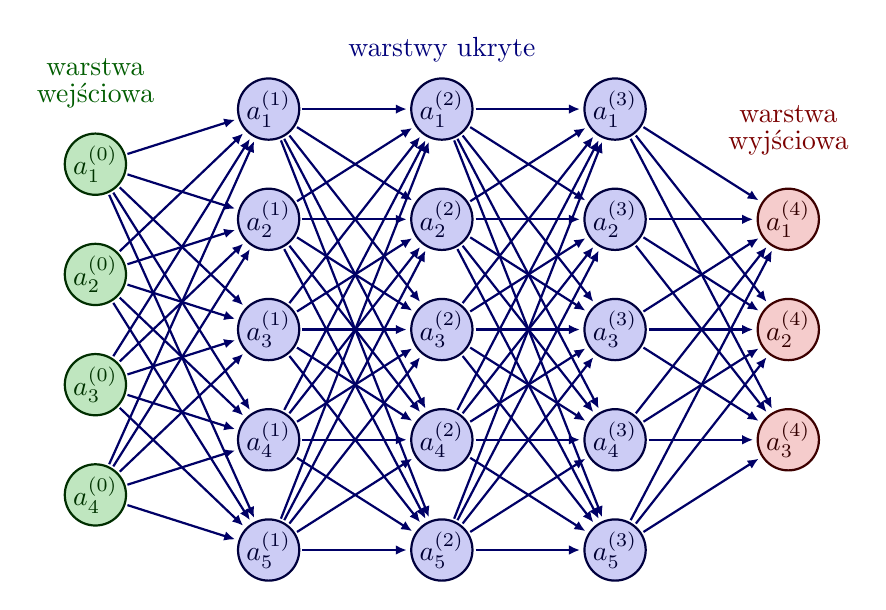
\begin{tikzpicture}[x=2.2cm,y=1.4cm]
	\message{^^JNeural network with arrows}
	\readlist\Nnod{4,5,5,5,3} % array of number of nodes per layer
	
	\message{^^J  Layer}
	\foreachitem \N \in \Nnod{ % loop over layers
		\edef\lay{\Ncnt} % alias of index of current layer
		\message{\lay,}
		\pgfmathsetmacro\prev{int(\Ncnt-1)} % number of previous layer
		\foreach \i [evaluate={\y=\N/2-\i; \x=\lay; \n=\nstyle;}] in {1,...,\N}{ % loop over nodes
			
			% NODES
			\node[node \n] (N\lay-\i) at (\x,\y) {$a_\i^{(\prev)}$};
			%\node[circle,inner sep=2] (N\lay-\i') at (\x-0.15,\y) {}; % shifted node
			%\draw[node] (N\lay-\i) circle (\R);
			
			% CONNECTIONS
			\ifnum\lay>1 % connect to previous layer
			\foreach \j in {1,...,\Nnod[\prev]}{ % loop over nodes in previous layer
				\draw[connect arrow] (N\prev-\j) -- (N\lay-\i); % connect arrows directly
				%\draw[connect arrow] (N\prev-\j) -- (N\lay-\i'); % connect arrows to shifted node
			}
			\fi % else: nothing to connect first layer
			
		}
		
	}

	  \node[above=5,align=center,mygreen!60!black] at (N1-1.90) {warstwa\\[-0.2em]wejściowa};
	\node[above=2,align=center,myblue!60!black] at (N3-1.90) {warstwy ukryte};
	\node[above=8,align=center,myred!60!black] at (N\Nnodlen-1.90) {warstwa\\[-0.2em]wyjściowa};
\end{tikzpicture}
\end{figure}

Sieci neuronowe, znane również jako sztuczne sieci neuronowe lub symulowane sieci neuronowe są częścią funkcji uczenia maszynowego i stanowią podstawę algorytmów uczenia głębokiego. Ich nazwa i struktura są wzorowane na ludzkim mózgu i naśladują sposób, w jaki biologiczne neurony komunikują się między sobą.

Sztuczne sieci neuronowe składają się z warstw węzłów, obejmujących warstwę wejściową, jedną lub więcej warstw ukrytych oraz warstwę wyjściową. Każdy węzeł (sztuczny neuron) łączy się z innym i ma powiązaną wagę oraz próg. Jeśli wyjście dowolnego pojedynczego węzła przekracza określoną wartość progową, węzeł ten jest aktywowany podczas wysyłania danych do kolejnej warstwy sieci. W przeciwnym razie żadne dane nie są przekazywane do następnej warstwy sieci.

\begin{figure}[h!]
	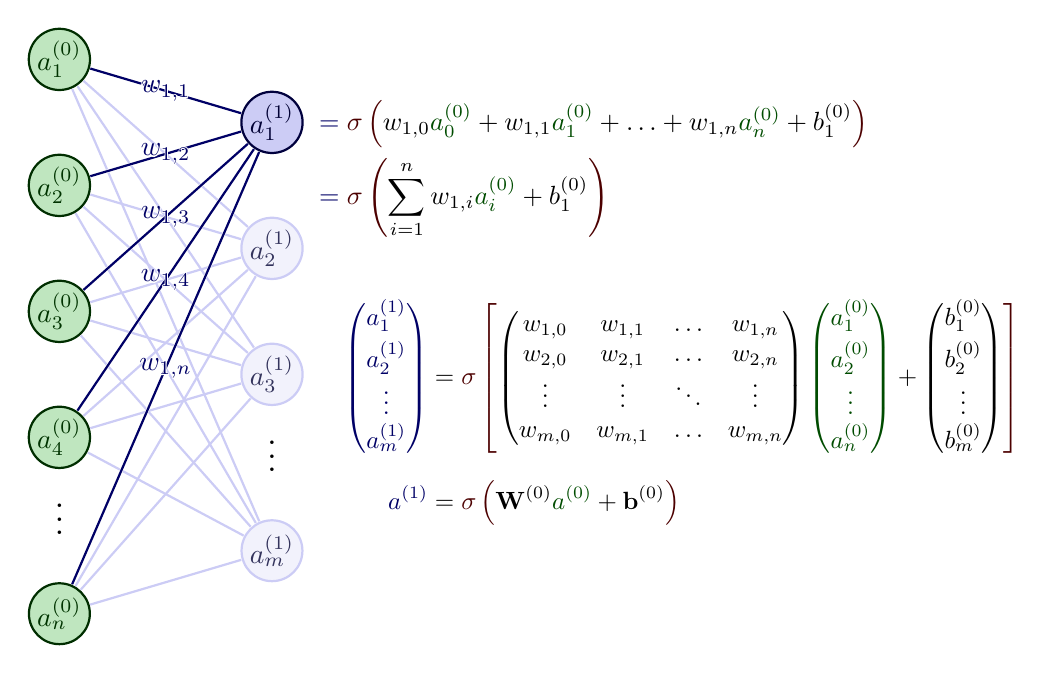
\begin{tikzpicture}[x=2.7cm,y=1.6cm]
		\message{^^JNeural network activation}
		\def\NI{5} % number of nodes in input layers
		\def\NO{4} % number of nodes in output layers
		\def\yshift{0.4} % shift last node for dots
		
		% INPUT LAYER
		\foreach \i [evaluate={\c=int(\i==\NI); \y=\NI/2-\i-\c*\yshift; \index=(\i<\NI?int(\i):"n");}]
		in {1,...,\NI}{ % loop over nodes
			\node[node in,outer sep=0.6] (NI-\i) at (0,\y) {$a_{\index}^{(0)}$};
		}
		
		% OUTPUT LAYER
		\foreach \i [evaluate={\c=int(\i==\NO); \y=\NO/2-\i-\c*\yshift; \index=(\i<\NO?int(\i):"m");}]
		in {\NO,...,1}{ % loop over nodes
			\ifnum\i=1 % high-lighted node
			\node[node hidden]
			(NO-\i) at (1,\y) {$a_{\index}^{(1)}$};
			\foreach \j [evaluate={\index=(\j<\NI?int(\j):"n");}] in {1,...,\NI}{ % loop over nodes in previous layer
				\draw[connect,white,line width=1.2] (NI-\j) -- (NO-\i);
				\draw[connect] (NI-\j) -- (NO-\i)
				node[pos=0.50] {\contour{white}{$w_{1,\index}$}};
			}
			\else % other light-colored nodes
			\node[node,blue!20!black!80,draw=myblue!20,fill=myblue!5]
			(NO-\i) at (1,\y) {$a_{\index}^{(1)}$};
			\foreach \j in {1,...,\NI}{ % loop over nodes in previous layer
				%\draw[connect,white,line width=1.2] (NI-\j) -- (NO-\i);
				\draw[connect,myblue!20] (NI-\j) -- (NO-\i);
			}
			\fi
		}
		
		% DOTS
		\path (NI-\NI) --++ (0,1+\yshift) node[midway,scale=1.2] {$\vdots$};
		\path (NO-\NO) --++ (0,1+\yshift) node[midway,scale=1.2] {$\vdots$};
		
		% EQUATIONS
		\def\agr#1{{\color{mydarkgreen}a_{#1}^{(0)}}}
		\node[below=17,right=11,mydarkblue,scale=0.95] at (NO-1)
		{$\begin{aligned} %\underset{\text{bias}}{b_1}
				&= \color{mydarkred}\sigma\left( \color{black}
				w_{1,0}\agr{0} + w_{1,1}\agr{1} + \ldots + w_{1,n}\agr{n} + b_1^{(0)}
				\color{mydarkred}\right)\\
				&= \color{mydarkred}\sigma\left( \color{black}
				\sum_{i=1}^{n} w_{1,i}\agr{i} + b_1^{(0)}
				\color{mydarkred}\right)
			\end{aligned}$};
		\node[right,scale=0.9] at (1.3,-1.3)
		{$\begin{aligned}
				{\color{mydarkblue}
					\begin{pmatrix}
						a_{1}^{(1)} \\[0.3em]
						a_{2}^{(1)} \\
						\vdots \\
						a_{m}^{(1)}
				\end{pmatrix}}
				&=
				\color{mydarkred}\sigma\left[ \color{black}
				\begin{pmatrix}
					w_{1,0} & w_{1,1} & \ldots & w_{1,n} \\
					w_{2,0} & w_{2,1} & \ldots & w_{2,n} \\
					\vdots  & \vdots  & \ddots & \vdots  \\
					w_{m,0} & w_{m,1} & \ldots & w_{m,n}
				\end{pmatrix}
				{\color{mydarkgreen}
					\begin{pmatrix}
						a_{1}^{(0)} \\[0.3em]
						a_{2}^{(0)} \\
						\vdots \\
						a_{n}^{(0)}
				\end{pmatrix}}
				+
				\begin{pmatrix}
					b_{1}^{(0)} \\[0.3em]
					b_{2}^{(0)} \\
					\vdots \\
					b_{m}^{(0)}
				\end{pmatrix}
				\color{mydarkred}\right]\\[0.5em]
				{\color{mydarkblue}a^{(1)}}
				&= \color{mydarkred}\sigma\left( \color{black}
				\mathbf{W}^{(0)} {\color{mydarkgreen}a^{(0)}}+\mathbf{b}^{(0)}
				\color{mydarkred}\right)
				%\color{black},\quad \mathbf{W}^{(0)} \in \mathbb{R}^{m\times n}
			\end{aligned}$};
		
	\end{tikzpicture}
\end{figure}

O każdym pojedynczym węźle należy myśleć jak o modelu regresji liniowej złożonym z danych wejściowych, wag, odchyleń (lub wartości progowych) i danych wyjściowych. Rysunek powyżej przedstawia właśnie te obliczenia dla jednego neurona. Macierz $\mathbf{W}^{(0)}$ jest macierzą wszystkich wag wchodzących do każdego neurona warstwy $a^{(0)}$ z warstwy poprzedniej, wektor $b^(0)$ to wartości wszystkich \textit{bias-ów} danej warstwy, a $\sigma$ to funkcja aktywacji danej warstwy.

Wagi pomagają określić znaczenie każdej zmiennej, przy czym większe z nich mają większy wpływ na wynik wyjściowy w porównaniu do innych danych wejściowych. Wszystkie dane wejściowe są następnie mnożone przez swoje odpowiednie wagi, a potem sumowane. Następnie wyniki są przepuszczane przez funkcję aktywacji, która określa wartość wyjściową.
	
\setcounter{subsection}{52}
\subsection{Deklaratywne programowanie w logice: klauzule Horne'a, nawracanie}
	Logika Hoare’a – formalizm matematyczny służący do opisu poprawności algorytmów.
	Trójka $\{P\}C\{Q\}$ oznacza, że fragment kodu $C$, o ile na wejściu będzie miał stan spełniający warunek $P$, oraz zakończy swoje działanie, to na wyjściu da stan spełniający warunek $Q$. Formułę $P$ nazywamy warunkiem wstępnym, a formułę $Q$ nazywamy warunkiem końcowym.\\
	
	Przykład:
	do instrukcji przypisania $x:=5$ możemy dopisać następujące warunki wstępne i końcowe:
		\begin{center}
				$\{{\text{true}}\}x:=5\{x=5\}$
		\end{center}
	co oznacza, że przy dowolnym stanie przed wykonaniem instrukcji, po wykonaniu instrukcji będziemy mieli stan, w którym zmiennej $x$ jest przypisana wartość 5.\\
	
	
	Prawdą jest też bardziej skomplikowana formuła:\\
	
	\begin{center}
		$\{x=y+z\}\{$if $x<y$ then $ z:=-z\}\{x\leq y+z\}$
	\end{center}
	
	
	
\end{document}
